% Options for packages loaded elsewhere
\PassOptionsToPackage{unicode}{hyperref}
\PassOptionsToPackage{hyphens}{url}
%
\documentclass[
]{article}
\usepackage{lmodern}
\usepackage{amssymb,amsmath}
\usepackage{ifxetex,ifluatex}
\ifnum 0\ifxetex 1\fi\ifluatex 1\fi=0 % if pdftex
  \usepackage[T1]{fontenc}
  \usepackage[utf8]{inputenc}
  \usepackage{textcomp} % provide euro and other symbols
\else % if luatex or xetex
  \usepackage{unicode-math}
  \defaultfontfeatures{Scale=MatchLowercase}
  \defaultfontfeatures[\rmfamily]{Ligatures=TeX,Scale=1}
\fi
% Use upquote if available, for straight quotes in verbatim environments
\IfFileExists{upquote.sty}{\usepackage{upquote}}{}
\IfFileExists{microtype.sty}{% use microtype if available
  \usepackage[]{microtype}
  \UseMicrotypeSet[protrusion]{basicmath} % disable protrusion for tt fonts
}{}
\makeatletter
\@ifundefined{KOMAClassName}{% if non-KOMA class
  \IfFileExists{parskip.sty}{%
    \usepackage{parskip}
  }{% else
    \setlength{\parindent}{0pt}
    \setlength{\parskip}{6pt plus 2pt minus 1pt}}
}{% if KOMA class
  \KOMAoptions{parskip=half}}
\makeatother
\usepackage{xcolor}
\IfFileExists{xurl.sty}{\usepackage{xurl}}{} % add URL line breaks if available
\IfFileExists{bookmark.sty}{\usepackage{bookmark}}{\usepackage{hyperref}}
\hypersetup{
  pdftitle={Rapport ITV},
  hidelinks,
  pdfcreator={LaTeX via pandoc}}
\urlstyle{same} % disable monospaced font for URLs
\usepackage[margin=1in]{geometry}
\usepackage{graphicx,grffile}
\makeatletter
\def\maxwidth{\ifdim\Gin@nat@width>\linewidth\linewidth\else\Gin@nat@width\fi}
\def\maxheight{\ifdim\Gin@nat@height>\textheight\textheight\else\Gin@nat@height\fi}
\makeatother
% Scale images if necessary, so that they will not overflow the page
% margins by default, and it is still possible to overwrite the defaults
% using explicit options in \includegraphics[width, height, ...]{}
\setkeys{Gin}{width=\maxwidth,height=\maxheight,keepaspectratio}
% Set default figure placement to htbp
\makeatletter
\def\fps@figure{htbp}
\makeatother
\setlength{\emergencystretch}{3em} % prevent overfull lines
\providecommand{\tightlist}{%
  \setlength{\itemsep}{0pt}\setlength{\parskip}{0pt}}
\setcounter{secnumdepth}{-\maxdimen} % remove section numbering
\usepackage{booktabs}
\usepackage{longtable}
\usepackage{array}
\usepackage{multirow}
\usepackage{wrapfig}
\usepackage{float}
\usepackage{colortbl}
\usepackage{pdflscape}
\usepackage{tabu}
\usepackage{threeparttable}
\usepackage{threeparttablex}
\usepackage[normalem]{ulem}
\usepackage{makecell}
\usepackage{xcolor}

\title{Rapport ITV}
\author{}
\date{\vspace{-2.5em}}

\begin{document}
\maketitle

\hypertarget{collected-data}{%
\subsection{Collected data}\label{collected-data}}

We have collected 36 answers.

\begin{table}[H]
\centering
\begin{tabular}{l|l|l|l|l|l|l|l|l|l|l|l|l|l|l|l|l|l|l|l|l|l|l|l|l|l|l|l|l|l|l|l|l|l|l|l|l|l|l|l|l|l|l|l|l|l|l|l|l|l|l}
\hline
ID & Heure de début & Heure de fin & Adresse de messagerie & Nom & Langue & Connaissez-vous quelqu'un qui a déjà fait un test COVID ? & Pensez-vous que les tests COVID en général sont douloureux ? & Quel test réalisez-vous le plus fréquemment ? & Prendre l'avion & Se rendre au travail & Se rendre à son lieu de formation & Voyager dans un autre pays (train, voiture, etc) & Voir des proches & Activités spécifiques (boites de nuit, compétitions sportives, etc) & Evènements (spéctacles, foires, etc) & Symptômes & Racontez-moi la dernière expérience que vous avez eu lorsque vous avez fait un test COVID ? & Coût & Facilité d'accès (proximité du domicile) & Délais entre la prise de rdv/achat et le test & Simplicité d'utilisation & Informations claires & Précision des résultats du test & Rapidité de la délivrance des résultats & Sentiment de sécurité & Certification et validité & Test PCR (\textasciitilde{}150 CHF) & Test antigénique avec certificat (\textasciitilde{}30 CHF) & Auto-Test après les 5 gratuits (10 CHF) & Test PCR (\textasciitilde{}150 CHF)2 & Test antigénique avec certificat (\textasciitilde{}30 CHF)2 & Auto-Test après les 5 gratuits (10 CHF)2 & Pour finir ... si vous aviez trois souhaits pour changer les choses lorsque vous vous faites tester, lesquels seraient-ils ? & Etape 1 : Rendez-vous & Etape 2 : Test & Etape 3 : Résultat & Pour quelle(s) raison(s) pourriez-vous utiliser cette nouvelle solution de test ? & Imaginez maintenant que vous vous trouvez dans la situation spécifique d'une nouvelle vague de COVID en octobre 2021, quelle(s) méthode(s) voudriez-vous utiliser pour vous faire tester ? & En faisant l'hypothèse que l'assurance ne paie pas, quel serait selon vous le prix CORRECT  pour cette nouvelle solution de test ? & En faisant l'hypothèse que l'assurance ne paie pas, quel serait le prix MAXIMAL que vous seriez prêt(e) à payer pour cette nouvelle solution de test ? & Très bien. Maintenant faites l'hypothèse que cette solution puisse être offerte à 100CHF/test. Quelle est la probabilité que vous la recommandiez à un ami(e) ou à un de vos proches ? & Expliquez votre choix : & Quel est votre âge & Sexe & Etes-vous vaccinés? & Extra: Commentaires & Autres & Prix & Connaître les variants & Quel est votre niveau de formation ?\\
\hline
1 & 7/30/21 15:16:03 & 7/30/21 15:23:57 & anonymous & 1 & Deutsch & Vous-même; & Plutôt non & PCR & 0 fois & 0 fois & 0 fois & 0 fois & 0 fois & 0 fois & 0 fois & 2 fois (environ une fois par semestre) &  & Sans avis & J'ai apprécié (+) & J'ai apprécié (+) & J'ai apprécié (+) & Sans avis & Sans avis & Sans avis & J'ai apprécié (+) & J'ai apprécié (+) & 2 fois &  & 2 fois & 2 fois &  &  &  & Équivalent aux tests que j'utilise actuellement & Équivalent aux tests que j'utilise actuellement & Plutôt meilleur que les tests que j'utilise actuellement & Se rendre à un évènement;Faire une activité spécifique; & Test antigénique; & 50 & 80 & 3 & Comme ce teste offre une meilleure précision, je le conseillerais seulement au personne à risque. & <20 ans & Homme & Oui &  &  &  &  & \\
\hline
2 & 7/30/21 15:32:46 & 7/30/21 15:42:27 & anonymous & 1 & Deutsch & Vous-même;Un.e de vos ami.e.s; & Neutre & test anti-genique & 0 fois & 0 fois & 1 fois (environ une fois par an) & 1 fois (environ une fois par an) & 0 fois & 0 fois & 0 fois & 0 fois & "Avant : recherche des laboratoires faisant le test Pendant: anxieux d'une possible contamination Après : attente du résultat par mail" & Je n'ai pas apprécié (-) & Je n'ai pas apprécié (-) & J'ai apprécié (+) & J'ai apprécié (+) & J'ai apprécié (+) & J'ai apprécié (+) & Sans avis & J'ai apprécié (+) & J'ai apprécié (+) & 1 fois & 4 fois & Jamais & Jamais & 2 fois & 2 fois & "Rapidité Simplicité " & Plutôt meilleur que les tests que j'utilise actuellement & Plutôt pire que les tests que j'utilise actuellement & Plutôt meilleur que les tests que j'utilise actuellement & Voir des proches;Faire une activité spécifique;Aller dans un autre pays;Aller sur le lieu de formation/d'étude; & Test PCR;Nouvelle solution de test;Test antigénique; & 80 & 100 & 7 & il m'est difficile de justifier que ce nouveau test est plus précis que le pcr car je n'ai pas l'information. & 21-30 ans & Homme & Oui &  &  &  &  & \\
\hline
3 & 44204.5922222222 & 44204.5958680556 & anonymous & 1 & Français (France) & Vous-même;Une personne de votre famille;Un.e de vos ami.e.s; & Plutôt oui & Test rapide & 1 fois (environ une fois par an) & 1 fois (environ une fois par an) & 1 fois (environ une fois par an) & 1 fois (environ une fois par an) & 0 fois & 0 fois & 1 fois (environ une fois par an) & 0 fois & Confirmation lenteur résultats peu rapide & Sans avis & J'ai apprécié (+) & J'ai apprécié (+) & Sans avis & Je n'ai pas apprécié (-) & Je n'ai pas apprécié (-) & Je n'ai pas apprécié (-) & Sans avis & Sans avis & Jamais & Jamais & 1 fois & 1 fois & 1 fois & 1 fois & X & Plutôt meilleur que les tests que j'utilise actuellement & Plutôt meilleur que les tests que j'utilise actuellement & Plutôt meilleur que les tests que j'utilise actuellement & Prendre l'avion;Aller dans un autre pays;Se rendre à un évènement; & Nouvelle solution de test;Auto-Test; & 50 & 50 & 5 & Trop cher & 41-50 ans & Femme & Oui &  &  &  &  & \\
\hline
4 & 44235.6200810185 & 44235.6257986111 & anonymous & 1 & Français (France) & Vous-même;Une personne de votre famille;Un.e de vos ami.e.s;Un.e collègue de travail; & Neutre & Antigénique & 0 fois & 0 fois & 0 fois & 1 fois (environ une fois par an) & 0 fois & 0 fois & 0 fois & 0 fois & La prise de rendez-vous s'est faite sur internet, ensuite j'ai imprimé les documents nécessaires avant de me rendre à l'endroit du test. Je suis rentrée dans le cabanon, j'ai donné les documents et la carte d'assurance maladie, elle m'a fait le test et ensuite je suis sortie. J'ai reçu le résultat par sms 20 minutes après et ensuite j'ai reçu les résultats par email (documents officiels à imprimer pour montrer la preuve du test aux frontières). & J'ai apprécié (+) & J'ai apprécié (+) & J'ai apprécié (+) & J'ai apprécié (+) & J'ai apprécié (+) & J'ai apprécié (+) & J'ai apprécié (+) & J'ai apprécié (+) & J'ai apprécié (+) & Jamais & 1 fois & 1 fois & Jamais & 2 fois & 4 fois & 1. qu'ils ne disent pas qu'on est positif alors qu'on n'a pas de symptômes, 2. qu'on sache directement les résultats et 3. qu'ils soient fiables & Équivalent aux tests que j'utilise actuellement & Équivalent aux tests que j'utilise actuellement & Plutôt meilleur que les tests que j'utilise actuellement & Prendre l'avion;Aller dans un autre pays; & Test antigénique;Auto-Test;Nouvelle solution de test; & 150 & 100 & 8 & Je la recommanderai car elle pourrait déterminer le variant mais je n'ai pas mis 9 ou 10 parce que d'autres tests peuvent indiquer si nous avons le COVID ou non & 21-30 ans & Femme & Non &  &  &  &  & \\
\hline
5 & 44235.6433333333 & 44235.6499189815 & anonymous & 1 & Deutsch & Vous-même;Une personne de votre famille;Un.e de vos ami.e.s;Un.e collègue de travail; & Plutôt oui & Test rapide/antigénique & 1 fois (environ une fois par an) & 0 fois & 0 fois & 1 fois (environ une fois par an) & 0 fois & 0 fois & 1 fois (environ une fois par an) & 0 fois & J'ai effectué un test pour partir en vacances. L'inscription sur internet était rapide et facile. Le résultat après le test prend seulement 15 minutes. & J'ai apprécié (+) & J'ai apprécié (+) & J'ai apprécié (+) & J'ai apprécié (+) & J'ai apprécié (+) & J'ai apprécié (+) & J'ai apprécié (+) & Sans avis & J'ai apprécié (+) & Jamais & 4 fois & Jamais & 1 fois & 2 fois & Jamais & "Possibilité de venir sans rendez-vous Validité plus longue Conseil sur la validité du certificat (géographiquement par exemple)" & Équivalent aux tests que j'utilise actuellement & Équivalent aux tests que j'utilise actuellement & Équivalent aux tests que j'utilise actuellement & Prendre l'avion;Aller travailler;Aller dans un autre pays;Faire une activité spécifique;Se rendre à un évènement; & Test antigénique;Nouvelle solution de test; & 40 & 100 & 7 & Si le nouveau test se veut plus pratique que les précédents et est valable plus longtemps, le prix peut se justifier. & 21-30 ans & Homme & Non &  &  &  &  & \\
\hline
6 & 44235.6751851852 & 44235.691099537 & anonymous & 1 & Deutsch & Vous-même;Une personne de votre famille;Un.e de vos ami.e.s;Un.e collègue de travail; & Plutôt oui & Antigénique & 0 fois & 0 fois & 0 fois & 1 fois (environ une fois par an) & 0 fois & 0 fois & 0 fois & 0 fois & "Avant : recherche de disponibilités compliquée, tout était complet en valais aux dates voulues Pendant : personnel à l'écoute, accueil agréable malgré un test douloureux Après : résultats rapides, informations précises et correctes au sujet du test" & J'ai apprécié (+) & J'ai apprécié (+) & Je n'ai pas apprécié (-) & Sans avis & J'ai apprécié (+) & J'ai apprécié (+) & Sans avis & J'ai apprécié (+) & J'ai apprécié (+) & Jamais & 1 fois & Jamais & Jamais & 1 fois & 1 fois & "- pouvoir se faire tester gratuitement, surtout pour partir à l'étranger - accès plus simple, prévoir plus de disponibilités lors des périodes de départs en vacances, car le délai d'attente est incroyablement long - test salivaire au lieu du nez" & Équivalent aux tests que j'utilise actuellement & Meilleur que les tests que j'utilise actuellement & Plutôt pire que les tests que j'utilise actuellement & Prendre l'avion;Aller dans un autre pays;Voir des proches;Se rendre à un évènement; & Auto-Test;Nouvelle solution de test; & 0 & 15 & 0 & Trop cher. C'est une contrainte et non un choix. Cela ne devrait donc pas être payant. & 21-30 ans & Femme & Oui &  &  &  &  & \\
\hline
\end{tabular}
\end{table}

Collected data shows that most people do not think that they should pay
for testing (the fair price for most people is below 50 CHF) . But when
asked what is the maximum amount they are willing to pay, a new cluster
emerges (Graph 02).\\
Indeed, some people are willing to pay 100 CHF for the new test, and
they are going to recommend it to other users (NPS).

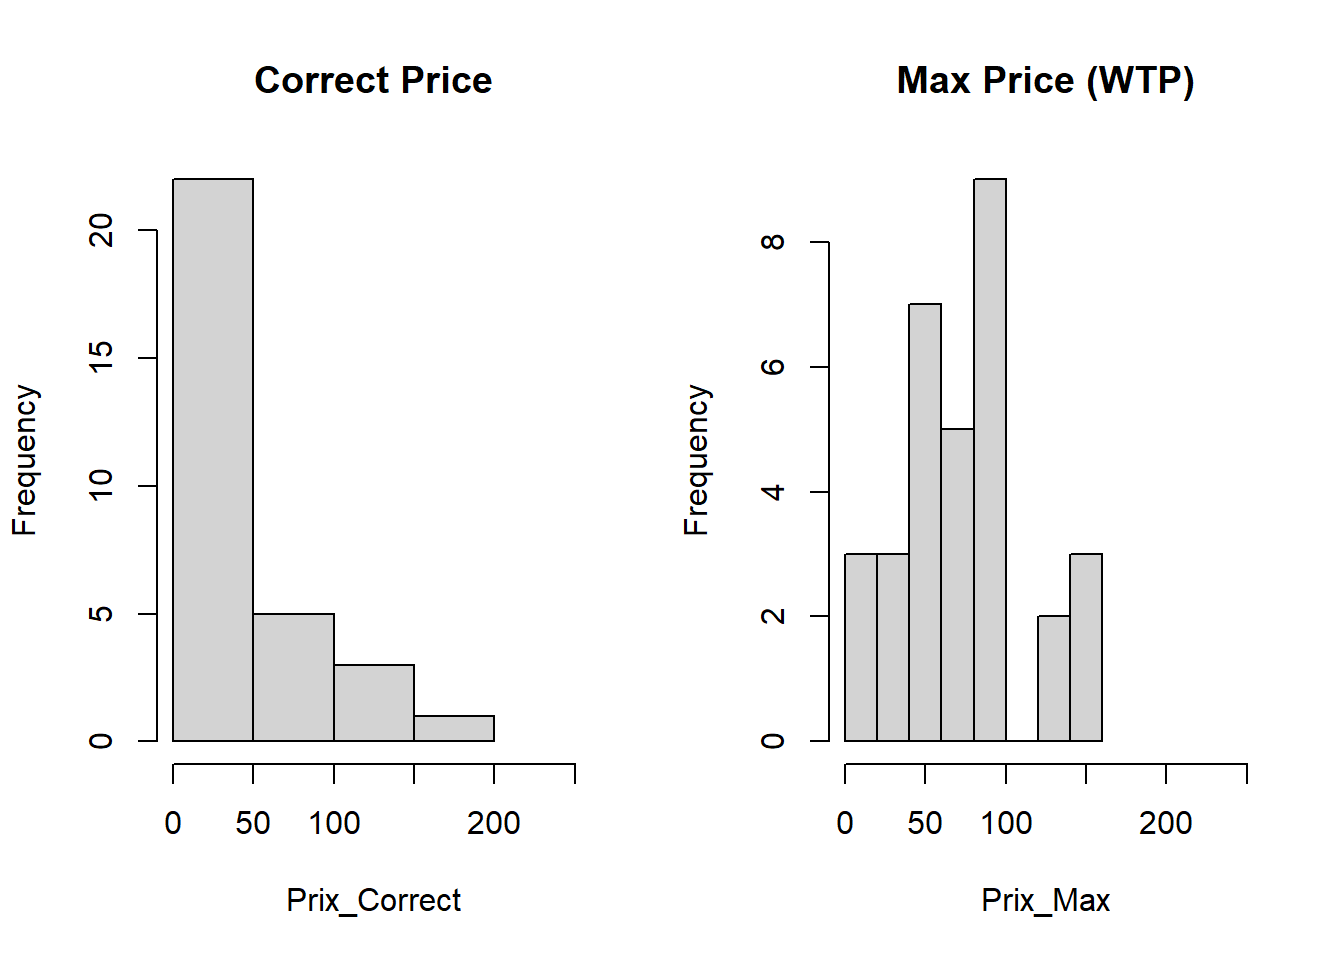
\includegraphics{RapportITV_files/figure-latex/unnamed-chunk-4-1.pdf}
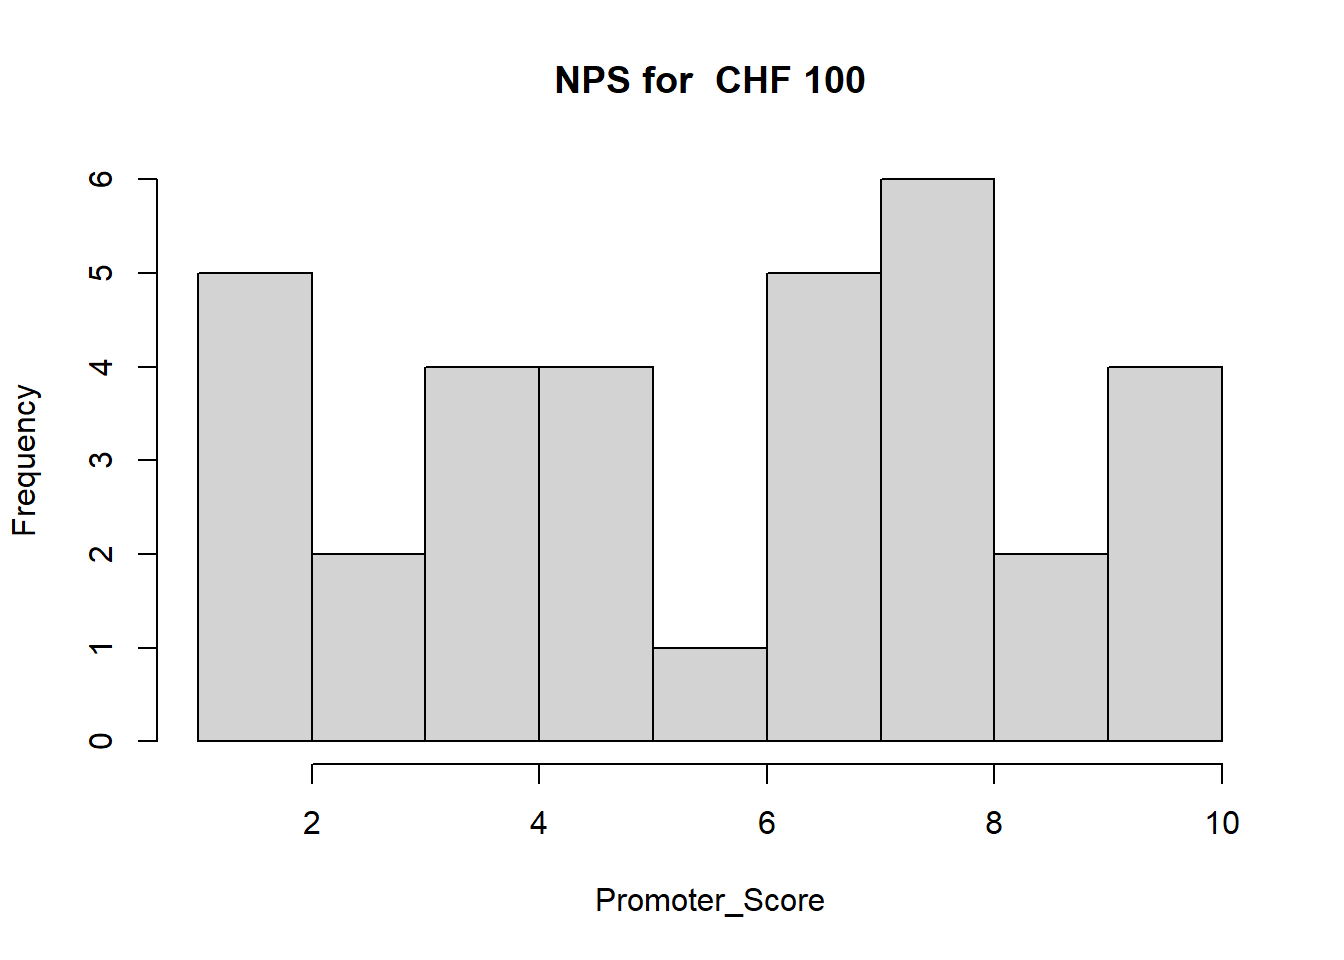
\includegraphics{RapportITV_files/figure-latex/unnamed-chunk-4-2.pdf}
\includegraphics{RapportITV_files/figure-latex/unnamed-chunk-4-3.pdf}
\newpage

\hypertarget{looking-for-champions}{%
\subsection{Looking for Champions}\label{looking-for-champions}}

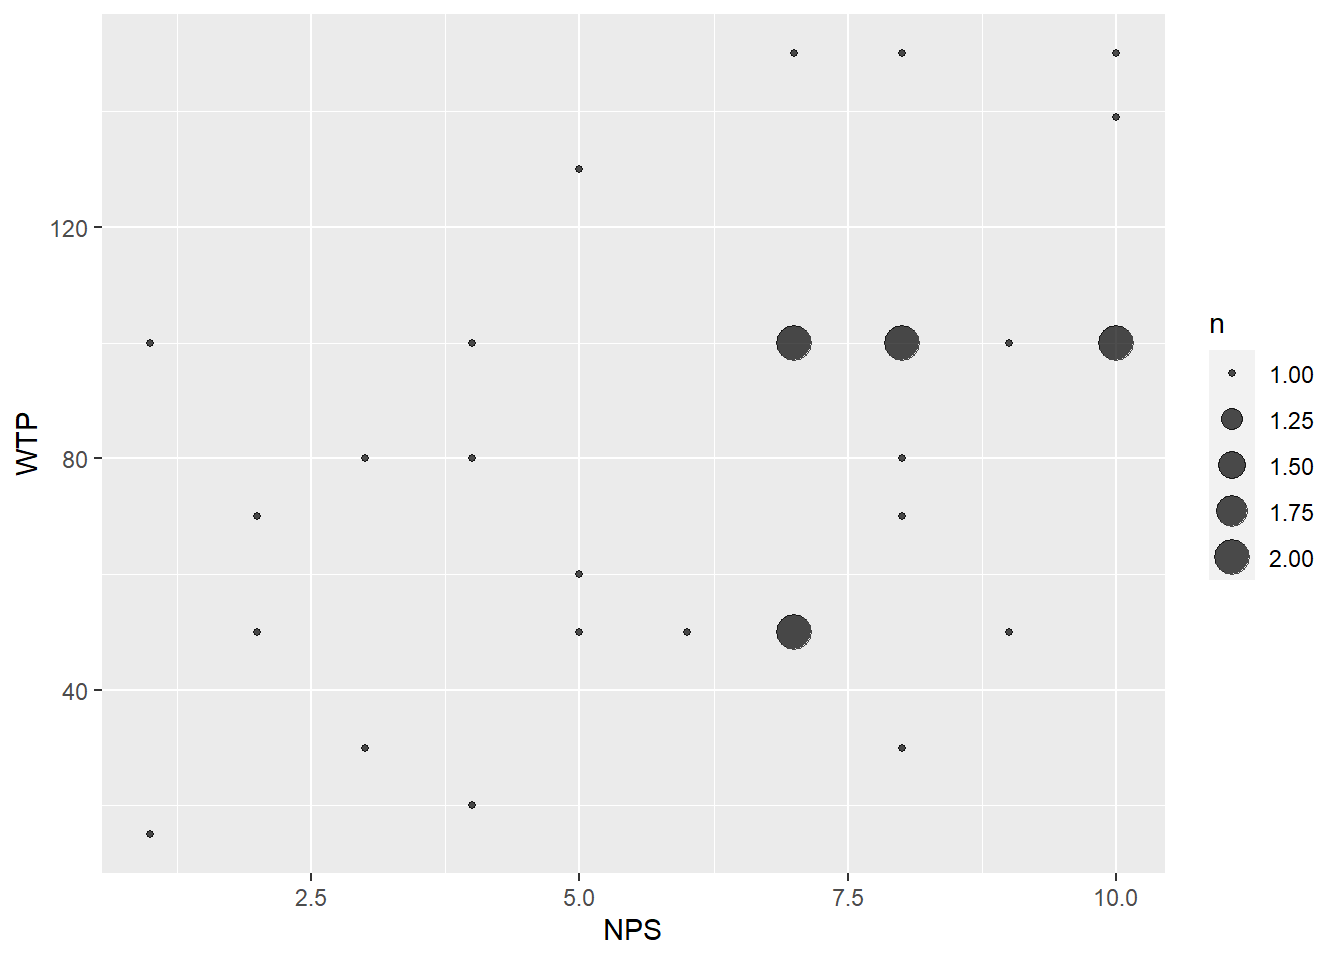
\includegraphics{RapportITV_files/figure-latex/unnamed-chunk-5-1.pdf}

So how can we predict if a customer is a good customer ?

We are currently looking for customers

\begin{itemize}
\item
  that are willing to pay at least 100 CHF and
\item
  that have an estimated probability to recommend our product of at
  least 7/10 (every customer with a score below 7 is considered a
  detractor)
\end{itemize}

After 2 rounds of interviews, we had 11 champions over a total of 36
respondents (=0.3\%).

\newpage

\hypertarget{exploratory-data-analysis-with-random-forest}{%
\subsection{Exploratory Data Analysis with Random
Forest}\label{exploratory-data-analysis-with-random-forest}}

In this section, the systems analyzes 70\% of the collected data (=0.7 *
36) and test its model to predict 10 answers.\\
The results are shown below.

\begin{table}[H]
\centering
\begin{tabular}{l|r|r|r|l}
\hline
.pred\_class & .pred\_Detractor & .pred\_Neutral & .pred\_Supporter & NPS\_Fact\\
\hline
Detractor & 0.742 & 0.084 & 0.174 & Detractor\\
\hline
Neutral & 0.382 & 0.614 & 0.004 & Neutral\\
\hline
Detractor & 0.802 & 0.078 & 0.120 & Detractor\\
\hline
Neutral & 0.230 & 0.768 & 0.002 & Neutral\\
\hline
Detractor & 0.602 & 0.398 & 0.000 & Detractor\\
\hline
Detractor & 0.722 & 0.170 & 0.108 & Detractor\\
\hline
Supporter & 0.378 & 0.058 & 0.564 & Supporter\\
\hline
Detractor & 0.904 & 0.016 & 0.080 & Detractor\\
\hline
Detractor & 0.654 & 0.184 & 0.162 & Detractor\\
\hline
Supporter & 0.252 & 0.154 & 0.594 & Supporter\\
\hline
\end{tabular}
\end{table}

The accuracy of the Random forest model is 1 (1.0 = 100\% being the
maximum).

The classification rules extracted by the system are \ldots{}

\begin{table}[H]
\centering
\begin{tabular}{l|l|l|l|l}
\hline
len & freq & err & condition & pred\\
\hline
3 & 0.04 & 0 & Before \%in\% c('Same','Worse') \& During \%in\% c('Worse') \& After \%in\% c('Better','Same') & Supporter\\
\hline
3 & 0.08 & 0 & Before \%in\% c('Same','Worse') \& During \%in\% c('Better') \& After \%in\% c('Better') & Neutral\\
\hline
1 & 0.08 & 0 & Before \%in\% c('Worse') & Neutral\\
\hline
2 & 0.16 & 0.25 & Before \%in\% c('Same','Worse') \& During \%in\% c('Better') & Neutral\\
\hline
1 & 0.2 & 0.4 & During \%in\% c('Better') & Neutral\\
\hline
2 & 0.08 & 0.5 & During \%in\% c('Worse') \& After \%in\% c('Better') & Neutral\\
\hline
2 & 0.08 & 0 & During \%in\% c('Same') \& After \%in\% c('Better') & Detractor\\
\hline
3 & 0.04 & 0 & Before \%in\% c('Better') \& During \%in\% c('Better') \& After \%in\% c('Better') & Detractor\\
\hline
2 & 0.16 & 0.25 & During \%in\% c('Better','Worse') \& After \%in\% c('Same','Worse') & Detractor\\
\hline
1 & 0.16 & 0.25 & Before \%in\% c('Better') & Detractor\\
\hline
3 & 0.32 & 0.375 & Before \%in\% c('Same') \& During \%in\% c('Same') \& After \%in\% c('Better','Worse') & Detractor\\
\hline
2 & 0.32 & 0.375 & Before \%in\% c('Better','Same') \& After \%in\% c('Worse') & Detractor\\
\hline
1 & 0.16 & 0.5 & During \%in\% c('Worse') & Detractor\\
\hline
3 & 0.44 & 0.545 & Before \%in\% c('Same','Worse') \& During \%in\% c('Better','Same') \& After \%in\% c('Better','Worse') & Detractor\\
\hline
3 & 0.2 & 0.6 & Before \%in\% c('Same') \& During \%in\% c('Same','Worse') \& After \%in\% c('Same') & Detractor\\
\hline
3 & 0.32 & 0.625 & Before \%in\% c('Same','Worse') \& During \%in\% c('Better','Same') \& After \%in\% c('Same') & Detractor\\
\hline
\end{tabular}
\end{table}

\newpage

\hypertarget{effect-of-the-customer-journey-on-promoter-score}{%
\subsection{Effect of the customer journey on promoter
score}\label{effect-of-the-customer-journey-on-promoter-score}}

The customer journey seems to have an effect on the willingness to pay
of the customers.\\
Nonetheless, the collected sample was fairly small and we predict what
is the probability that the results could change, if new data is
collected.

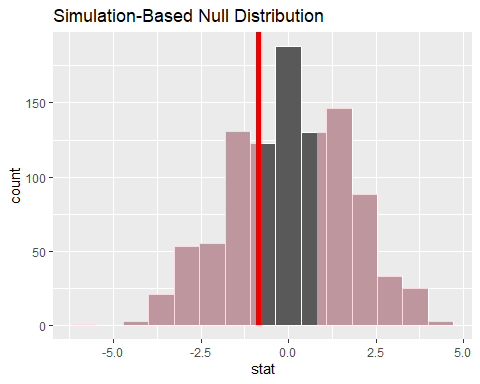
\includegraphics{RapportITV_files/figure-latex/unnamed-chunk-10-1.pdf}

The probability that the difference between the NPS scores of those who
liked the new ``Before'' stage (wrt those who did not like it) will
change, if new data is collected, is: 0.29 (p-value).

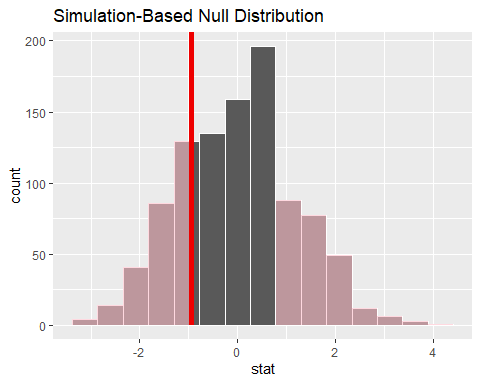
\includegraphics{RapportITV_files/figure-latex/unnamed-chunk-11-1.pdf}

The probability that the difference between the NPS scores of those who
liked the new ``DUring'' stage or thought it was the same (wrt those who
did not like it) will change, if new data is collected, is: 0.63
(p-value)

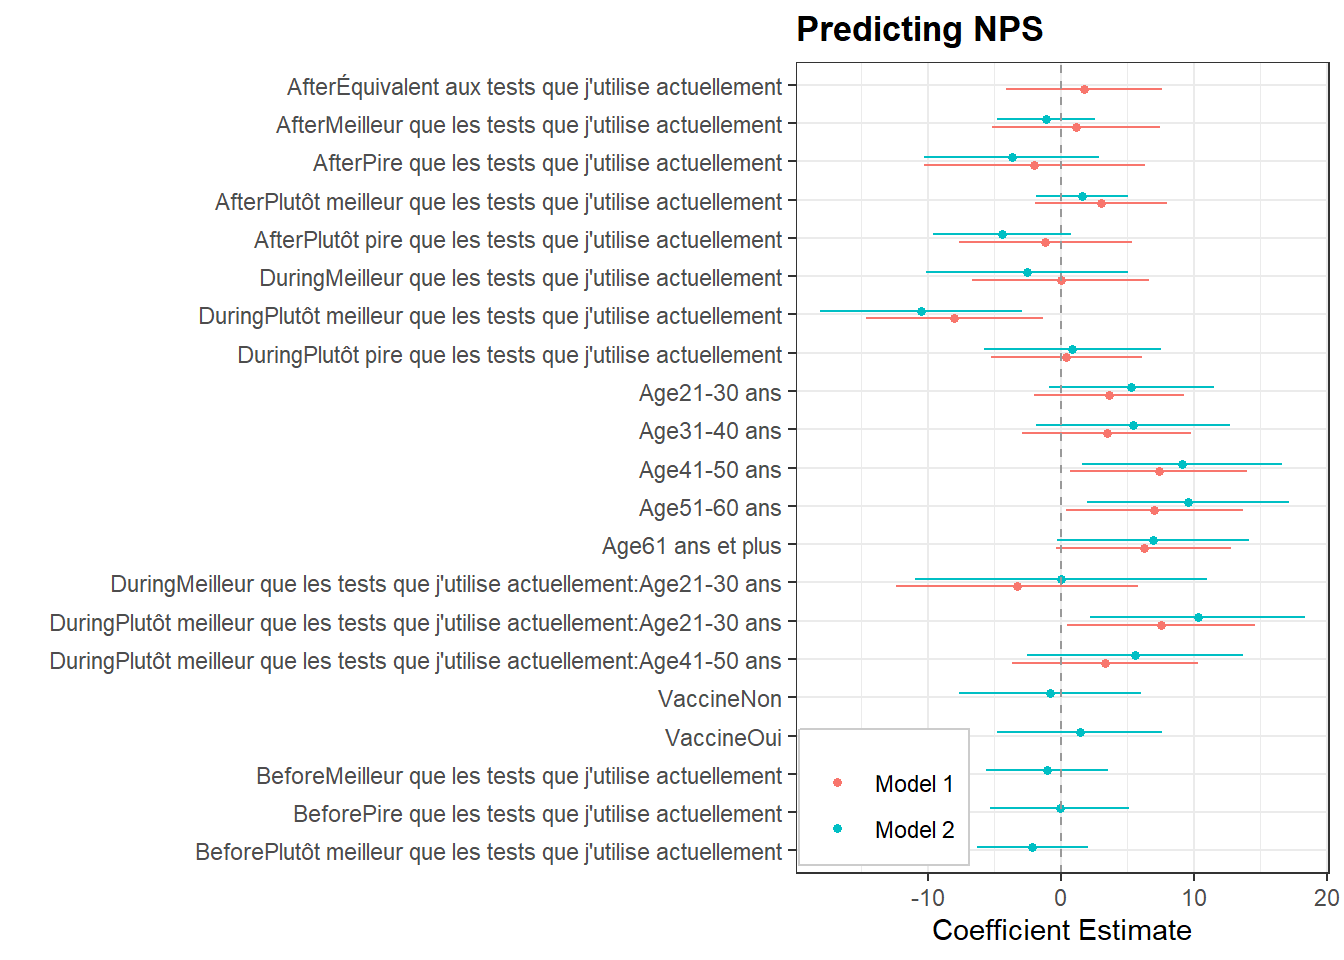
\includegraphics{RapportITV_files/figure-latex/unnamed-chunk-12-1.pdf}

The probability that the difference between the NPS scores of those who
liked the new ``After'' stage (wrt those who did not like it) will
change, if new data is collected, is: 0.47 (p-value)

\hypertarget{effect-of-the-customer-journey-on-the-nps-associated-with-100-chf}{%
\subsection{Effect of the customer journey on the NPS associated with
100
CHF}\label{effect-of-the-customer-journey-on-the-nps-associated-with-100-chf}}

\begin{table}[H]
\centering
\begin{tabular}{l|r|r|r|r}
\hline
term & estimate & std.error & statistic & p.value\\
\hline
Age<20 ans & -1.0714286 & 2.751585 & -0.3893859 & 0.7007344\\
\hline
Age21-30 ans & 2.9075988 & 1.093686 & 2.6585320 & 0.0143506\\
\hline
Age31-40 ans & 2.4748734 & 1.743772 & 1.4192643 & 0.1698361\\
\hline
Age41-50 ans & 8.4986829 & 1.605817 & 5.2924364 & 0.0000260\\
\hline
Age51-60 ans & 7.4360182 & 1.495734 & 4.9714845 & 0.0000565\\
\hline
Age61 ans et plus & 7.4360182 & 1.495734 & 4.9714845 & 0.0000565\\
\hline
TestExperienceBetter & -9.5074468 & 2.974678 & -3.1961263 & 0.0041700\\
\hline
TestExperienceWorse & -1.5074468 & 2.974678 & -0.5067596 & 0.6173651\\
\hline
TestResultsBetter & 3.0714286 & 1.264735 & 2.4285160 & 0.0237882\\
\hline
TestResultsWorse & -1.2480243 & 1.150307 & -1.0849492 & 0.2896907\\
\hline
Age21-30 ans:TestExperienceBetter & 9.3569909 & 3.184645 & 2.9381579 & 0.0076077\\
\hline
Age31-40 ans:TestExperienceBetter &  &  &  & \\
\hline
Age41-50 ans:TestExperienceBetter & 2.7104863 & 3.416931 & 0.7932516 & 0.4361035\\
\hline
Age51-60 ans:TestExperienceBetter &  &  &  & \\
\hline
Age61 ans et plus:TestExperienceBetter &  &  &  & \\
\hline
Age21-30 ans:TestExperienceWorse & -0.0079534 & 3.410107 & -0.0023323 & 0.9981601\\
\hline
Age31-40 ans:TestExperienceWorse &  &  &  & \\
\hline
Age41-50 ans:TestExperienceWorse &  &  &  & \\
\hline
Age51-60 ans:TestExperienceWorse &  &  &  & \\
\hline
Age61 ans et plus:TestExperienceWorse &  &  &  & \\
\hline
\end{tabular}
\end{table}

The linear regression analysis shows that respondents \emph{aged
\textgreater40} have the tendency to give at least 7/10 for the NPS
(p\textless0.01).\\
If the \emph{Test result} phase is perceived as better than the current
one, the scores goes up 3 points (p\textless0.05). An loss in quality of
\emph{Testing phase} leads to 1 point less, whereas an improvement in
the \emph{Testing phase} in itself seems to be more problematic to
understand: if respondents have less somewhere between 21 and 30 years,
there is not effect (-9.5 + 9.35). Instead, if they are aged between 41
and 50 years old, the score might be going down 7 points
(p\textgreater0.40).

Although the model has many variables its explanatory power is fairly
good: the Adjusted R2 of the model is 0.41.

\newpage

\hypertarget{appendix-correct-price}{%
\subsection{Appendix: Correct price}\label{appendix-correct-price}}

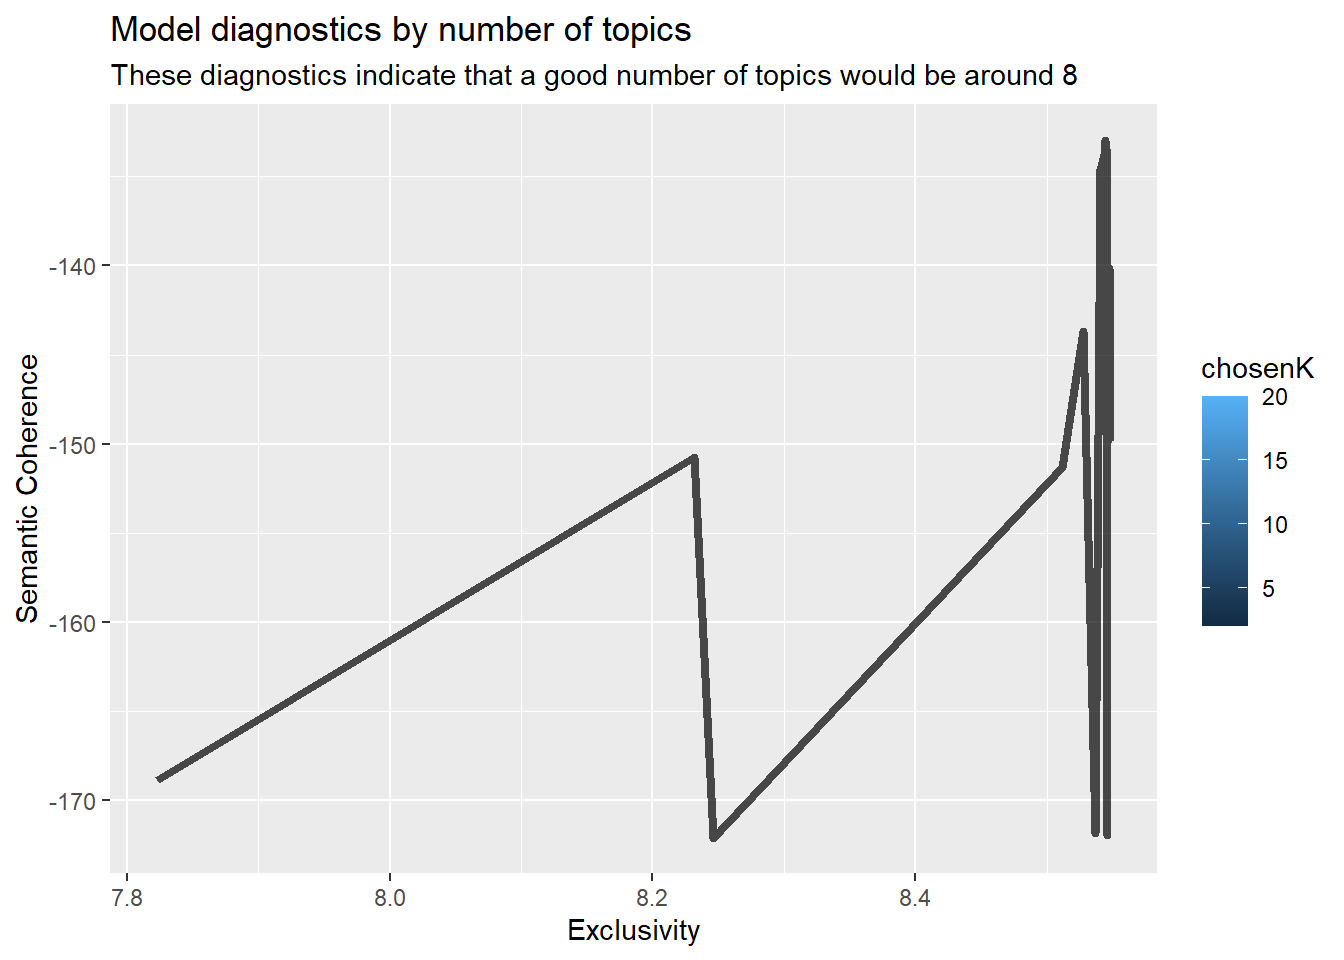
\includegraphics{RapportITV_files/figure-latex/unnamed-chunk-16-1.pdf}

\begin{itemize}
\item
  La courbe bleue montre les prix corrects de la nouvelle solution qu'on
  partagé les sondés tandis que la courbe orange montre les prix
  maximaux qu'ils seraient prêts à débourser pour une telle solution
\item
  Nous remarquons que la grande majorité des sondés ont défini des prix
  maximaux qui se trouvent en dessous des prix qu'ils trouvent corrects
  pour une telle solution.
\item
  La moyenne des prix corrects estimés par le panel est de : CHF
\item
  La moyenne des prix maximaux estimés par le panel est de : CHF
\item
  La différence moyenne entre la perception de ces deux prix est
  d'environ : CHF
\end{itemize}

\end{document}
